% This is based on the LLNCS.DEM the demonstration file of
% the LaTeX macro package from Springer-Verlag
% for Lecture Notes in Computer Science,
% version 2.4 for LaTeX2e as of 16. April 2010
%
% See http://www.springer.com/computer/lncs/lncs+authors?SGWID=0-40209-0-0-0
% for the full guidelines.
%

\documentclass{llncs}

\usepackage[noend]{algpseudocode}
\usepackage{algorithm}

\usepackage{amsmath}
\usepackage{tikz}
\usepackage{tkz-graph}

\usetikzlibrary{decorations.markings}

\newcommand{\zero}{\mathrm{zero}}
\newcommand{\const}{\mathrm{const}}
\newcommand{\afin}{\mathrm{affine\ in\ }}
\newcommand{\linin}{\mathrm{linear\ in\ }}

\DeclareMathOperator{\Perm}{Perm}
\DeclareMathOperator{\Conj}{Conj}
\DeclareMathOperator{\SimultConj}{SimultConj}
\DeclareMathOperator{\len}{length}

% \title{Improving PBE by Verifying Robustness Properties}
\title{Verifying Robustness of Programs Under Algebraic Perturbations}
\author{Jacob Bond and Clay Thomas}
\institute{Purdue University}

\begin{document}

\maketitle 

% \begin{abstract}
% \end{abstract}

\section{Introduction}

% continuity is no longer the focus; this introduction needs to be modified
It is desirable for programs to respond smoothly to changes in input, in the sense that if a small change is made to the input, the change in output is also small.  Many classical algorithms are indeed robust with respect to continuity \cite{chaudhuri11}.  In the setting of PBE, a user would likely prefer, and expect, a program synthesizer to return a robust program.  For this reason, the ability to efficiently verify robustness would be useful in the determination of which program the synthesizer should return.

Moreover, a synthesizer which returns robust programs will itself be more robust.  Let \(\mathcal{I}_{1} = (I_{1}, O_{1})\) and \(\mathcal{I}_{2} = (I_{2}, O_{2})\) be two input-output pairs for a program synthesizer which differ by a small perturbation.  If the program \(\mathcal{P}_{1}\) returned by the synthesizer on input \(\mathcal{I}_{1}\) is robust, then \(\mathcal{P}_{1}(I_{2})\) will approximate \(O_{2}\) because \(I_{2}\) approximates \(I_{1}\).  For this reason, \(\mathcal{P}_{2}\), the program returned on input \(\mathcal{I}_{2}\), should only differ from \(\mathcal{P}_{1}\) by a small amount.

Finally, if a sufficiently efficient method for verifying program robustness is developed, it could be applied to a program synthesizer in order to verify directly that the synthesizer is indeed robust.

\subsection{Motivating Example}

Consider an attempt to specify the \(\max\) function by providing to the synthesizer \(\Big((13, 15), 15\Big)\), \(\Big((-23, 19), 19\Big)\), and \(\Big((-75, -13), -13\Big)\).  In order to synthesize a simpler program, the result would likely be a program which returns the second argument.  However, if instructed to return a program which is invariant under permuting the arguments, this would no longer be a viable program, and it is likely that the synthesizer would return a function for finding the \(\max\) of two elements.

Moreover, by reversing the inputs from the input-output pairs given above, the synthesizer would now be likely to construct a program which returns the first input.  In this way, the synthesizer is sensitive to small changes in input, and would not be robust itself.

\subsection{Problem Definition}

% discuss k-safety properties here
Our goal is to formulate robustness conditions inside of a first-order theory, in order to utilize an SMT solver in checking robustness.  In particular, we will explore various robustness properties for arrays of integers, as well as automated methods for checking these properties with an SMT solver.  We will perform an experiment to determine the improvements that result from a synthesis engine being able to reason about robustness properties.

\section{Robustness Properties}

Robustness of a program is the property that the program behaves predictably on uncertain inputs \cite{chaudhuri12}.  In our context, the uncertainty derives from the fact that the user's input only specifies a very small number of potential arguments to the desired function and that the returned program should not change drastically as a result of specifying input-output pairs which are slightly perturbed.

Some settings in which programs should be robust:
\begin{itemize}
\item numerical perturbations \cite{samanta14,chaudhuri10,chaudhuri11},
\item permutations of arrays,
\item simultaneous permutations of arrays,
\item relabeling of inputs \cite{zapponi03}.
\end{itemize}

\paragraph{Robustness as a 2-Safety Property}
A 2-safety property is one which requires reasoning about two execution traces simultaneously.  As robustness requires reasoning about uncertain inputs, this can be achieved by considering a given input along with a second input which may be considered to vary over the range of uncertainty.  In this way, robustness is a 2-safety property.

\section{Preliminaries}

\subsection{Continuity and Lipschitz-Continuity}

% define continuity and LIpschitz-continuity of a program

\subsection{Permutations}
\label{perms}

A permutation is a bijection from a set \(\Omega\) to itself \cite{dummitfoote}.  When \(\Omega\) is a finite set, a permutation can be specified using two-line notation by placing the elements of \(\Omega\) on one line, and their images under \(\sigma\) beneath them:

% increase the intercolumn spacing
\begin{center}
\begin{tabular*}{0.5\textwidth}{c@{\extracolsep{\fill}}c}
\(\sigma\):
\begin{tabular}{cccccc}
0 & 1 & 2 & 3 & 4 & 5\\
5 & 2 & 3 & 1 & 4 & 0
\end{tabular}
&
\(\sigma\):
\begin{tabular}{ccc}
a & b & c\\
a & c & b
\end{tabular}
\end{tabular*}
\end{center}

Similar to two-line notation, a permutation on \(\{0, \dotsc, N-1\}\) can be encoded in an array \(a\) of length \(N\) by placing the image of \(i\) in \(a[i]\).  The example \(\sigma\) above is encoded in an array as \(\sigma = [5, 2, 3, 1, 4, 0]\), so that \(\sigma(i) = \sigma[i]\).

The inverse \(\sigma^{-1}\) of a permutation \(\sigma\) is the permutation defined by
\[\sigma(i) = j \Longleftrightarrow \sigma^{-1}(j) = i.\]
For the permutation \(\sigma\) above,
\[\sigma^{-1}:\begin{tabular}{cccccc}
0 & 1 & 2 & 3 & 4 & 5\\
5 & 3 & 1 & 2 & 4 & 0
\end{tabular}.\]

% give first-order formula for being a permutation
\paragraph{First-Order Formula for a Permutation}
The property of being a permutation on \(\{0, \dotsc, N-1\}\) is encoded in the theory of arrays as
\begin{multline*}\Perm(a, N): N = \len(a) \wedge (\forall i. 0 \leq i < N \rightarrow 0 \leq a[i] < N) \wedge\\(\forall i,j. 0 \leq i < j < N \rightarrow a[i] \not= a[j]).\end{multline*}

\paragraph{Action on an Array}

Given a permutation \(\sigma\), \(\sigma\) can {\it act} on an array \(a\) as follows.  Let \(a = [37, 25, 19, 49, 81, 21]\) and \(\sigma\) be as above.  Then \(\sigma(3) = \sigma[3] = 1\) and applying \(\sigma\) to \(a\) results in the element of \(a\) at index \(3\), \(49\), being moved to index \(1\) in \(\sigma a\).  That is, \(\sigma a[1] = 49\) and \(a[3] = \sigma a[1] = \sigma a[\sigma[3]]\).  More generally,
\[\sigma a[\sigma[i]] = a[i] \Longleftrightarrow \sigma a[i] = a[\sigma^{-1}[i]].\]

\paragraph{Generating Permutations}
For information on permutation groups, see \S1.3 in \cite{dummitfoote}.

\makeatletter
\renewcommand{\@cite}[1]{#1}
\makeatother
The permutations on \(N\) elements, \(S_{N}\), can all be expressed as compositions of the permutations [Exercises 3-4, \S3.5, \cite{dummitfoote}]

% increase the intercolumn spacing
\[\begin{tabular}{ccccc}
0 & 1 & 2 & \(\dotsm\) & \(N-1\)\\
1 & 0 & 2 & \(\dotsm\) & \(N-1\)
\end{tabular}
\qquad\textrm{and}\qquad
\begin{tabular}{ccccc}
0 & 1 & 2 & \(\dotsm\) & \(N-1\)\\
1 & 2 & 3 & \(\dotsm\) & 0
\end{tabular}.\]
\makeatletter
\renewcommand{\@cite}[1]{[#1]}
\makeatother

\section{Examples of Robust Programs}

\subsection{Continuity}

% discuss sorting being 1-Lipschitz

\subsection{Permutations}

Suppose \(\mathcal{P}\) is a program with takes an array as input.  Assume further that it is desired that \(\mathcal{P}\) be permutation invariant.

\subsubsection{Sorting}



% discuss maximum function being invariant under permutations

\subsubsection{Searching}

% discuss that if P(a, x) finds x in the array a, then P(sigma(a), x) = sigma(P(a, x))

\subsubsection{Adjacency Matrices}

% programs operating on adjacency matrices should either be invariant under permutations or behave similarly to searching

\subsection{Further Examples of Robustness Properties}

\paragraph{Simultaneous Permutation}
Consider an algorithm for grading a multipart homework problem, which takes as input three arrays:  the student's responses, the correct answers, and the amounts that each part is worth.  A reordering of the parts of the problem should not affect the points which a student earns.  As reordering the parts of the problem corresponds to simultaneously permuting the three input arrays, the grading algorithm should be invariant under simultaneous permutations of the input arrays.  Using ideas from Section \ref{perms}, this property can be expressed as the conjunction of the following two formulas:

\begin{multline*}x_{2}[1] = x_{1}[0] \wedge y_{2}[1] = y_{1}[0] \wedge z_{2}[1] = z_{1}[0] \wedge\\
x_{2}[0] = x_{1}[1] \wedge y_{2}[0] = y_{1}[1] \wedge z_{2}[0] = z_{1}[1] \wedge\\
\forall i.\, 2 \leq i < \len(y_{1}) \rightarrow (x_{2}[i] = x_{1}[i] \wedge y_{2}[i] = y_{1}[i] \wedge z_{2}[i] = z_{1}[i])
\end{multline*}
\begin{multline*}\len(y_{1}) = N \wedge (x_{2}[0] = x_{1}[N-1] \wedge y_{2}[0] = y_{1}[N-1] \wedge z_{2}[0] = z_{1}[N-1]) \wedge\\ \forall i.\, 1 \leq i < N \rightarrow (x_{2}[i] = x_{1}[i-1] \wedge y_{2}[i] = y_{1}[i-1] \wedge z_{2}[i] = z_{1}[i-1])
\end{multline*}
%\begin{multline*}N = \len(y_{1}) \wedge \exists a. \Perm(a, N) \wedge \forall i. 0 \leq i < N \rightarrow\\(x_{2}[a[i]] = x_{1}[i] \wedge y_{2}[a[i]] = y_{1}[i] \wedge z_{2}[a[i]] = z_{1}[i])\end{multline*}

\begin{algorithm}
\begin{algorithmic}
\Function{Grade}{responses, answers, credits}
\State points \(\gets\) 0
\For{0 \(\leq\) i \(\leq\) length(answers)}
\If{responses[i] \(-\) answers[i] \(=\) 0}
\State points \(\gets\) points \(+\) credits[i]
\EndIf
\EndFor
\Return{points}
\EndFunction
\end{algorithmic}
\end{algorithm}

% should this part actually be included?
\paragraph{Relabeling}
Consider a bipartite graph drawn without edge-crossings.  Labeling the edges results in a cyclic ordering of the edges around each vertex, which can then be viewed as a pair of permutations \(\sigma_{0}, \sigma_{1} \in S_{N}\).  However, relabeling the edges does not change the structure of the graph, and as such, many computations performed on the graph should be invariant under a relabeling of the graph.

\begin{figure}[h]
    \centering
    \begin{minipage}{0.5\textwidth}
        \centering
    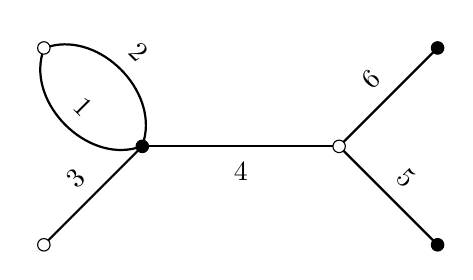
\begin{tikzpicture}
        \GraphInit[vstyle=Classic]
        \SetVertexMath
        \tikzset{
            VertexStyle/.style = {
                inner sep = 0pt,
                outer sep = 0pt,
                shape = circle,
                fill = black,
                minimum size = 4.5pt,
                draw}
                }
        \SetGraphUnit{1.25}
    \tikzset{VertexStyle/.append style={fill = white}}
    \Vertex[NoLabel = true]{A}
    \tikzset{VertexStyle/.append style={fill = black}}
    \SOEA[NoLabel = true](A){B}
    \tikzset{VertexStyle/.append style={fill = white}}
    \SOWE[NoLabel = true](B){C}
        {\SetGraphUnit{2.5}
        \EA[NoLabel = true](B){D}}
    \tikzset{VertexStyle/.append style={fill = black}}
    \SOEA[NoLabel = true](D){E}
    \NOEA[NoLabel = true](D){F}
    \SetUpEdge[labelstyle = {sloped,below = 2}]
        \Edge[label = 4](B)(D)
    \SetUpEdge[labelstyle = {sloped,above = 2}]
    \Edge[label = 3](B)(C)
        \Edge[label = 5](D)(E)
        \Edge[label = 6](D)(F)
    \tikzset{EdgeStyle/.append style = {bend left = 60}}
        \Edge[label = 1](B)(A)
        \Edge[label = 2](A)(B)
    \end{tikzpicture}
\end{minipage}\begin{minipage}{0.5\textwidth}
\begin{align*}
    \sigma_{0} &= (1\,3\,4\,2)(5)(6)\\
    \sigma_{1} &= (1\,2)(3)(4\,5\,6)
\end{align*}
\end{minipage}
\caption{A dessin d'enfant and its corresponding pair of permutations}
\end{figure}

A relabeling of the graph corresponds to simultaneously conjugating the permutations \(\sigma_{0}, \sigma_{1}\) by and element of \(S_{N}\).  This can be expressed in a first-order theory as follows:

\begin{enumerate}
\item Let the property that \(c\) conjugates \(a\) into \(b\) be given by
\[\Conj(a, b, c): \forall i.\, 0 \leq i < \len(a) \rightarrow a[c[i]] = c[b[i]].\]
\item Then being simultaneously conjugate is the property that
\[\SimultConj([x_{1}, y_{1}], [x_{2}, y_{2}]): \exists c.\, \Perm(c) \wedge \Conj(x_{1}, x_{2}, c) \wedge \Conj(y_{1}, y_{2}, c)\]
\end{enumerate}

An example of such an algorithm is to compute a canonical pair of permutations for any equivalence class of graphs.

\begin{algorithm}
\begin{algorithmic}[1]
\Function{CanonicalPair}{s0, s1}
\State CandidateReps \(\gets\) []
\For{0 \(\leq\) i \(<\) N}
\State \(Q \gets \) Deque([i]), perm \(\gets\) [i]
\While{length(perm) \(<\) N}
\State \(x\gets\) PopLeft(Q)
\For{s in (s0, s1)}
\If{s(x) not in perm}
\State Append(perm, s(x))
\State PushRight(Q, s(x))
\EndIf
\EndFor
\EndWhile
\State Append(CandidateReps,[perm\(^{-1}\)\(*\)s0\(*\)perm, perm\(^{-1}\)\(*\)s1\(*\)perm])
\EndFor
\Return{Min(CandidateReps)}
\EndFunction
\end{algorithmic}
\end{algorithm}

\section{Verifying Robustness Using Cartesian Hoare Logic}

% discuss using Descartes' algorithm to verify robustness

\subsection{Shortcomings Regarding Lipschitz-Continuity}

% discuss how the If rule of CHL can be improved for verifying continuity

\section{Preliminaries}

\subsection{The symetric group}
The symetric group $S_n$ is the group of bijective functions on the set $\{1,2,\ldots, n\}$, which we call permutations. We will write elements of $S_n$ using ``cycle notation'', where $(i_1\ i_2\ \ldots\ i_m)$ represents the permutation that sends $i_j$ to $i_{j+1}$ for $j=1,\ldots, m-1$ and sends $i_m$ to $i_1$.

We will often talk about the symmetric group acting on linear data types (namely, arrays, lists, and strings). For any $\sigma \in S_n$ and any array $a$, this action is given by the formula
$$ (\sigma a)[i] = a[\sigma(i)] $$
where we index our arrays starting at $1$. This action extends naturally to lists and strings. For an example, the action of the full cycle $(1\ 2\ 3\ \ldots\ n)$ just ``rotates'' a string by one, e.g. $(1\ 2\ 3\ 4)``abcd'' = ``bcda''$.
% discuss the use of arrays for representing permutations maybe?

\subsection{Automata}
We consider two classes of automata: finite state machines (FSM) and finite state transducers (FST). All automata we consider are deterministic. Given an automata $A$, we denote by $A(s)$ the output of $A$ on input $s$. If $A$ is an FSM, we represent "accept" by $1$ and "reject" by $0$. Otherwise, $A$ is a finite state transducer (FST), and $A(s)$ is a string. For a FSM $A$, let $L(A)$ denote the set of strings accepted by $A$. (We do not define the language of an FST).

Recall that for any FSMs $A$ and $B$, the problem of determining whether $L(A) = L(B)$ is decidable. We can compose an FST $T$ and a FSM $A$, denoted $A \circ T$, to get another FSM. 

We will assume that all input strings are terminated by a special end-of-input character \$.

\section{Invariance under permuting lists}
\label{permlists}

A different problem we have been thinking about is more discrete
and algebraic in nature.
We want to verify that programs are invariant under
permutations of their input arrays.

\subsection{Automata}
Given a program $P$ which takes a linear data type
as input. We may wish to verify that this program
is invariant under reordering of the array,
in other words, it is invariant under the action of $S_n$.
Denote the output of $P$ on input $s$ by $P(s)$.
Then we want to test whether $P(\sigma s) = P$
for all $\sigma \in S_n$.

As a first simplification, observe that is
suffices to check our condition on a set
of generators of $S_n$.
Concretely, let $\alpha = (1\ 2\ 3\ ...\ n)$
and let $\beta = (1\ 2)$.
Then any $\sigma \in S_n$ can be written as
a product of elements of $\{\alpha,\beta\}$,
say $\sigma = u_1 u_2\ldots u_m$ with
$u_i \in \{\alpha,\beta\}$.
So if we know that $P(\alpha s) = P(s)$
and $P(\beta s) = P(s)$, then
$P((u_1 u_2 \ldots u_m)s)
= P((u_2 \ldots u_m)s)
= \ldots = P(u_ms) = P(s) $.

For a fixed $n$ and $\sigma \in S_n$,
we can construct a finite state transducer
$T$ such that $T(s) = \sigma s$ for $|s|=n$.
However, this does not give us any
reasonable way of checking that a given
finite state machine is invariant under permutation
of the input string.
Instead, we will construct finite state
transducers $T_{\alpha}$ and $T_{\beta}$
such that for any $n$ and any string $s$ 
with $|s|=n$, we have 
$T_{\alpha}(s)=(1\ 2\ \ldots\ n) s$ and
$T_{\beta}(s) = (1\ 2) s$.
Then, determining whether an FSM $M$ is
invariant under permutation of its inputs
is equivalent to determining whether
\[ 
  L(M \circ T_\alpha) = L(M) = L(M \circ T_\beta)
\]

We now construct $T_\alpha$.
For each symbol $a \in \Sigma$,
$T_\alpha$ has a transition from its start
state $s_0$ to $s_a$, while reading in put $a$ and 
writing $\epsilon$ output.
For each $a$ and each $b\ne \$$, there is a
transition from $s_a$ to $s_a$, reading $b$
and writing $b$.
Then for each $a$, there is a transition from 
$s_a$ to $s_1$, reading $\$$ and writing $a\$$.

We now construct $T_\beta$.
For each symbol $a \in \Sigma$,
$T_\alpha$ has a transition from its start
state $s_0$ to $s_a$, while reading in put $a$ and 
writing $\epsilon$ output.
Each $s_a$ has a transition to $s_1$ while
reading input $b$ (for any $b\in \Sigma$)
and writing output $ba$.
Then $s_1$ simply has transitions to $s_1$,
reading any $a\in \Sigma$ and writing
back $a$.

\iffalse % maybe put this back in later
\subsection{Programs}
The previous section indicates a method for verifying
robustness of more general programs under permutation of inputs. 
% The framework of \cite{sousa16} is constructed in order to verify properties of related runs of the same program. However, their proof rules also give
Given a procedure $F$ taking an array as argument, consider the functions $F_\alpha$, which first swaps the first two elements of the array, then computes $F$, and $F_\beta$, which moves the first element of the array to the back, then computes $F$. Then $F$ is invariant under permutation of its input if and only if $F$ is functionally equivalent to $F_\alpha$ and $F_\beta$.

Certainly this method is more efficient than checking invariance under a larger class of permutations. For DFAs, this simplification made the problem of permutation invariance solvable. This indicates that this simplification may aid in our analysis in a profound way. For example, this may be a much easier way of verifying this invariance compared to expressing permutations as a general $2$-safety property.
\fi

\section{Invariance under permuting binary search trees}

In the previous section~\ref{permlists}, we found a reduction

\begin{algorithm}
\begin{algorithmic}[1]
\Function{Listify}{T}
\While{T has a right child}
  \State apply $\rho^{-1}$ to T
\EndWhile
\While{T has a left child}
  \While{T's left child has a right child}
    \State apply $\theta$ to T
  \EndWhile
  \State apply $\rho$ to T
\EndWhile
\EndFunction
\end{algorithmic}
\end{algorithm}

\section{Invariance with respect to a function}

\section{Related Work}

\subsection{Robustness}

Robustness for control systems was investigated by Majumdar and Saha \cite{majumdar09} and for general programs by \cite{chaudhuri11}.  Additionally, the robustness of networked systems was explored by Samanta et al. \cite{samanta13a}.

\subsection{Continuity}

Hamlet \cite{hamlet02} considered the concept of program continuity, but declared that automating verification of continuity for programs with loops was infeasible.  Chaudhuri et al. \cite{chaudhuri10,chaudhuri11} consider the continuity and Lipschitz continuity of programs over the real numbers. Samanta et al. \cite{samanta13} and Henzinger et al. \cite{samanta14} investigate the use of Lipschitz continuity for proving robustness in the context of transducers.

\subsection{\(k\)-safety Properties}

The concept of a 2-safety property was introduced by Terauchi and Aiken \cite{terauchi05} in the study of secure information flow.  Clarkson and Schneider \cite{clarkson08} introduced \(k\)-safety properties as a generalization of this idea.  Finally, Sousa and Dillig \cite{sousa16} formulated a verification algorithm in order to automate checking of \(k\)-safety properties.

%
% ---- Bibliography ----
%
\bibliographystyle{splncs}
\bibliography{robustness}

\end{document}

%\titlerunning{Verifying Alegebraic Proper} 
% abbreviated title (for running head)
% also used for the TOC unless \toctitle is used
%\authorrunning{Ivar Ekeland et al.} % abbreviated author list (for running head)
%%%% list of authors for the TOC (use if author list has to be modified)
%\tocauthor{Ivar Ekeland, Roger Temam, Jeffrey Dean, David Grove,
%Craig Chambers, Kim B. Bruce, and Elisa Bertino}
%\email{I.Ekeland@princeton.edu},\\ WWW home page:
%\texttt{http://users/\homedir iekeland/web/welcome.html}
%\and
%Universit\'{e} de Paris-Sud,
%Laboratoire d'Analyse Num\'{e}rique, B\^{a}timent 425,\\
%F-91405 Orsay Cedex, France}
